
\documentclass{article}

\usepackage{fancyhdr}
\usepackage{extramarks}
\usepackage{amsmath}
\usepackage{amsthm}
\usepackage{amsfonts}
\usepackage{tikz}
\usepackage[plain]{algorithm}
\usepackage{algpseudocode}
\usepackage{listings}
\usepackage{booktabs}
\usepackage{xcolor}
\usepackage[english]{babel}
\usepackage[T1]{fontenc}
\usepackage{lmodern,mathrsfs}
\usepackage{xparse}
\usepackage[inline,shortlabels]{enumitem}
\setlist{topsep=2pt,itemsep=2pt,parsep=0pt,partopsep=0pt}
\usepackage[dvipsnames]{xcolor}
\usepackage[utf8]{inputenc}
\usepackage[a4paper,top=0.5in,bottom=0.2in,left=0.5in,right=0.5in,footskip=0.3in,includefoot]{geometry}
\usepackage[most]{tcolorbox}
\tcbuselibrary{minted} % tcolorbox minted library, required to use the "minted" tcb listing engine (this library is not loaded by the option [most])
\usepackage{minted} % Allows input of raw code, such as Python code
% \usepackage[colorlinks]{hyperref}


\usetikzlibrary{automata,positioning}

\tcbset{
    pythoncodebox/.style={
        enhanced jigsaw,breakable,
        colback=gray!10,colframe=gray!20!black,
        boxrule=1pt,top=2pt,bottom=2pt,left=2pt,right=2pt,
        sharp corners,before skip=10pt,after skip=10pt,
        attach boxed title to top left,
        boxed title style={empty,
            top=0pt,bottom=0pt,left=2pt,right=2pt,
            interior code={\fill[fill=tcbcolframe] (frame.south west)
                --([yshift=-4pt]frame.north west)
                to[out=90,in=180] ([xshift=4pt]frame.north west)
                --([xshift=-8pt]frame.north east)
                to[out=0,in=180] ([xshift=16pt]frame.south east)
                --cycle;
            }
        },
        title={#1}, % Argument of pythoncodebox specifies the title
        fonttitle=\sffamily\bfseries
    },
    pythoncodebox/.default={}, % Default is No title
    %%% Starred version has no frame %%%
    pythoncodebox*/.style={
        enhanced jigsaw,breakable,
        colback=gray!10,coltitle=gray!20!black,colbacktitle=tcbcolback,
        frame hidden,
        top=2pt,bottom=2pt,left=2pt,right=2pt,
        sharp corners,before skip=10pt,after skip=10pt,
        attach boxed title to top text left={yshift=-1mm},
        boxed title style={empty,
            top=0pt,bottom=0pt,left=2pt,right=2pt,
            interior code={\fill[fill=tcbcolback] (interior.south west)
                --([yshift=-4pt]interior.north west)
                to[out=90,in=180] ([xshift=4pt]interior.north west)
                --([xshift=-8pt]interior.north east)
                to[out=0,in=180] ([xshift=16pt]interior.south east)
                --cycle;
            }
        },
        title={#1}, % Argument of pythoncodebox specifies the title
        fonttitle=\sffamily\bfseries
    },
    pythoncodebox*/.default={}, % Default is No title
}

% Custom tcolorbox for Python code (not the code itself, just the box it appears in)
\newtcolorbox{pythonbox}[1][]{pythoncodebox=#1}
\newtcolorbox{pythonbox*}[1][]{pythoncodebox*=#1} % Starred version has no frame

% Basic Document Settings
\topmargin=-0.45in
\evensidemargin=0in
\oddsidemargin=0in
\textwidth=6.5in
\textheight=9.0in
\headsep=0.25in
\linespread{1.1}

\pagestyle{fancy}
\lhead{\hmwkAuthorName}
\chead{\hmwkClass\ (\hmwkClassInstructor): \hmwkTitle}
\rhead{\firstxmark}
\lfoot{\lastxmark}
\cfoot{\thepage}
\renewcommand\headrulewidth{0.4pt}
\renewcommand\footrulewidth{0.4pt}
\setlength\parindent{0pt}

% Homework Details
\newcommand{\hmwkTitle}{Exam 1}
\newcommand{\hmwkDueDate}{Octubre 27, 2025}
\newcommand{\hmwkClass}{ESMA 6787}
\newcommand{\hmwkClassInstructor}{Israel Almodovar}
\newcommand{\hmwkAuthorName}{\textbf{Alejandro Ouslan}}

% Title Page
\title{
	\vspace{2in}
	\textmd{\textbf{\hmwkClass:\ \hmwkTitle}}\\
	\normalsize\vspace{0.1in}\small{Due\ on\ \hmwkDueDate}\\
	\vspace{0.1in}\large{\textit{\hmwkClassInstructor}}
	\vspace{3in}
}

\author{\hmwkAuthorName}
\date{}


% Begin document
\begin{document}
\maketitle
\pagebreak
\tableofcontents
\pagebreak

% Homework problem 1
\section*{Problem 1: Definitions}
Define the followings:
\begin{enumerate}[(a)]
	\item p-value:It is the probability that we would see that our results given that we asume that the null hypothesis is true
	\item Projection Matrix: It is the map of our estimated parameter and data onto the response variable. In other words is the
	      estimation of our fitted line
	\item Complete randomized Design: It is an experiment design were we randomly assign treatments to a sample.
	\item Complete Randomized Block Design: Similar to the CRD but with the distinction of partitioning the sample in shared characteristic

\end{enumerate}

\section*{Problem 2: Dough Experiment}
In the experiment to study the effects of the amount of baking powder in a biscuit dough upon the rise heights of the biscuits, four
levels of baking powder were tested and four replicate biscuits  were made with each level in a random order.
\begin{table}[!ht]
	\centering
	\caption{Training Methods Data}
	\begin{tabular}{c c c c}
		\hline
		\textbf{0.25 tsp} & \textbf{0.5 tsp} & \textbf{0.75 tsp} & \textbf{1 tsp} \\
		\hline
		11.4              & 27.8             & 47.6              & 61.6           \\
		11.0              & 29.2             & 47.0              & 62.4           \\
		11.3              & 26.8             & 47.3              & 63.0           \\
		9.5               & 26.0             & 45.5              & 63.9           \\
		\hline
	\end{tabular}
\end{table}
\begin{enumerate}[(a)]
	\item What is the experimental unit?

	      \textbf{Answer:} The biscuits dough
	\item Under this model  show why each of the following is estimable or non-estimable:
	      $$
		      \tau_1, \tau_2, \tau_3,\tau_4, \quad \tau_1 + \tau_2 - (\tau_3 + \tau_4), \mu + \tau_1 + \tau_2
	      $$
	      The overall model is given by the following:
	      $$
		      Y_{ij} = \mu + \tau_i + \epsilon_{ij}
	      $$
	      Thus:
	      \begin{enumerate}
		      \item $\tau_1 + \tau_2 -(\tau_3 + \tau_4$ Is also estimable given it is a also a linear combination
		      \item $\mu + \tau_1 + \tau_2$ is also estimable given it is a also a linear combination
	      \end{enumerate}
	\item Preform the analysis of variance to test the hypothesis of no treatment effect.
	      \begin{table}[!ht]
		      \centering
		      \caption{ANOVA for the Effect of Baking Powder on Biscuit Rise Height}
		      \begin{tabular}{lrrrrr}
			      \hline
			      \textbf{Source} & \textbf{df} & \textbf{Sum of Squares} & \textbf{Mean Square} & \textbf{F-statistic} & \textbf{p-value}         \\
			      \hline
			      BakingPowder    & 3           & 6145.73                 & 2048.58              & 1822.65              & \(3.23 \times 10^{-16}\) \\
			      Residual        & 12          & 13.49                   & 1.12                 & -                    & -                        \\
			      \hline
		      \end{tabular}
	      \end{table}

	\item Formulate a contrast to test the hypothesis that increase in rise height is a linear function of the increase in baking powder in the dough,
	      and test this hypothesis.

	      Choosing $L = -3\tau_1 -1\tau_2 + 1 \tau_3 + 3 \tau_3$ with the hypothesis:
	      \begin{enumerate}
		      \item $H_0$: no linear
		      \item $H_1$: linear
	      \end{enumerate}
	      \begin{table}[!ht]
		      \centering
		      \caption{ANOVA for the Effect of Baking Powder on Biscuit Rise Height and Linear Trend}
		      \begin{tabular}{lrrrrr}
			      \hline
			      \textbf{Source}          & \textbf{df} & \textbf{Sum of Squares} & \textbf{Mean Square} & \textbf{F-statistic} & \textbf{p-value}       \\
			      \hline
			      Treatment (BakingPowder) & 3           & 6145.732                & 2048.577             & 1822.645             & $3.23 \times 10^{-16}$ \\
			      Linear Trend             & 1           & 6137.256                & 6137.256             & 3912.062             & $1.54 \times 10^{-18}$ \\
			      Residual                 & 12          & 13.488                  & 1.124                & -                    & -                      \\
			      \hline
		      \end{tabular}
	      \end{table}
	      Withe the p-value we reject the null hypothesis and say that there exists a linear relationhsip between Rise and amount of baking powder

	\item If the dough were made in batches and the four replicate biscuit rise heights in each column (Table 1) were all from the same batch, would your answer to (a) be different?
	      How could the data be analyzed if this were the case?

	      \textbf{Answered:} The answer would be the same if would now have a batch effect. We could use latin squares for this experiments if it is structured in batches
\end{enumerate}

\section*{Problem 3: Rndomize grouop}

Consider a completely randomized design with four treatment groups, in which a total of $N = 100$
units are to be used. Although it won’t be explicitly used in the analysis model, treatments 1 through
5 actually represent increasing concentrations of one component in an otherwise standard chemical
compound, and the primary purpose of the experiment is to understand whether certain measurable
properties of the compound change with this concentration. The investigator decides to address these
questions by estimating these quantities
$$
	\tau_2 -\tau_1, \tau_2-\tau_3, \tau_2-\tau_4,\tau_3 - \tau_4, \tau_3-\tau_1
$$
where each $\tau_i$ is a parameter in the standard effects model. Find the optimal allocation for the 100
available units (i.e., values for $n1,\cdots, n5$) that minimizes the average variance of estimates of the five
contrasts of interest. Do this as a constrained, continuous optimization problem, then round the solution
to integer values that are consistent with the required constraints.

Consider a completely randomized design with five treatments and a total of $N = 100$ experimental units. We are interested in the following five contrasts:

\[
	\tau_2 -\tau_1, \quad \tau_2-\tau_3, \quad \tau_2-\tau_4, \quad \tau_3 - \tau_4, \quad \tau_3-\tau_1
\]

Where $\tau_i$ are the treatment effects in the standard effects model.


\[
	\begin{aligned}
		\mathrm{Var}(\tau_2-\tau_1) & = \sigma^2 \left( \frac{1}{n_1} + \frac{1}{n_2} \right) \\
		\mathrm{Var}(\tau_2-\tau_3) & = \sigma^2 \left( \frac{1}{n_2} + \frac{1}{n_3} \right) \\
		\mathrm{Var}(\tau_2-\tau_4) & = \sigma^2 \left( \frac{1}{n_2} + \frac{1}{n_4} \right) \\
		\mathrm{Var}(\tau_3-\tau_4) & = \sigma^2 \left( \frac{1}{n_3} + \frac{1}{n_4} \right) \\
		\mathrm{Var}(\tau_3-\tau_1) & = \sigma^2 \left( \frac{1}{n_3} + \frac{1}{n_1} \right)
	\end{aligned}
\]
\[
	V_{\text{avg}} \propto \frac{2}{n_1} + \frac{3}{n_2} + \frac{3}{n_3} + \frac{2}{n_4}.
\]

\[
	f(n_1,n_2,n_3,n_4) = \frac{2}{n_1} + \frac{3}{n_2} + \frac{3}{n_3} + \frac{2}{n_4}
\]
subject to
\[
	n_1 + n_2 + n_3 + n_4 + n_5 = 100, \quad n_i > 0.
\]

\[
	n_1 = n_4 = \sqrt{\frac{2}{\lambda}}, \quad n_2 = n_3 = \sqrt{\frac{3}{\lambda}},
\]
\[
	2\sqrt{\frac{2}{\lambda}} + 2\sqrt{\frac{3}{\lambda}} = 100 \implies \sqrt{\lambda} = \frac{\sqrt{2}+\sqrt{3}}{50}.
\]
\[
	n_1 = n_4 \approx 22.5, \quad n_2 = n_3 \approx 27.5, \quad n_5 \approx 0.
\]

\begin{table}[h]
	\centering
	\begin{tabular}{cccccc}
		\toprule
		Treatment   & 1  & 2  & 3  & 4  & 5 \\
		\midrule
		Units $n_i$ & 22 & 28 & 28 & 22 & 0 \\
		\bottomrule
	\end{tabular}
\end{table}


\section{Problem 4}

The effect of plant growth regulators and spear bud scales on spear elongation in asparagus
was investigated by Yang-Gyu and Woolley (2006). Elongation rate of spears is an important factor
determining final yield of asparagus in many temperate climatic conditions. Spears were harvested
from 6-year-old Jersey Giant asparagus plants grown in a commercial planting at Bulls (latitude 40.2S,
longitude 175.4E), New Zealand. Spears were harvested randomly and transported from field to lab
for investigation. After trimming to 80mm length, spears were immersed completely for 1 h in aqueous
solutions of 10 mg l-1 concentration of indole-3-acetic acid (IAA), abscisic acid (ABA), GA3, or CPPU
(Sitofex EC 2.0\%; SKW, Trostberg, Germany) in test tubes. Control spears were submerged in distilled
water for 1 h. The experiment was a completely randomized design with five replications (spears) per
treatment
\begin{table}[!ht]
	\centering
	\caption{Spear length in mm}
	\begin{tabular}{c c c c c c}
		\hline
		\textbf{Control} & \textbf{IAA} & \textbf{ABA} & \textbf{GA3} & \textbf{CPPU} \\
		\hline
		94.7             & 89.9         & 96.8         & 99.1         & 104.4         \\
		96.1             & 94.0         & 87.8         & 95.3         & 98.9          \\
		86.5             & 99.1         & 89.1         & 94.6         & 98.9          \\
		98.5             & 92.8         & 91.1         & 93.1         & 106.5         \\
		94.9             & 99.4         & 89.4         & 95.7         & 104.8         \\
		\hline
	\end{tabular}
\end{table}

\begin{enumerate}[(a)]
	\item What are the experimental units?
	      \textbf{Answer:} spear bud scales on spear elongation in asparagus are the experimental unit
	\item Proposed a linear model in this case. Explain each of the variable carefully.
	      Explain each of the terms carefully in context of the problem
	      $$
		      Y_{ij}= \mu + \tau_i + \epsilon_{ij}
	      $$
	      \begin{enumerate}
		      \item $Y_{ij}$: The spear length
		      \item $\mu$: the overall mean of the spear length
		      \item $\tau_i$: effect of the treatments
		      \item $\epsilon$: is the error term o unobserved effects
	      \end{enumerate}
	\item Test the hypothesis of no treatment effect. State the alternative, decision rule, and conclusion.
	      \begin{enumerate}
		      \item $H_0$: All treatments have the same effects of the spear length
		      \item $H_1$: At least one treatment has an effect
	      \end{enumerate}

	      \begin{table}[!ht]
		      \centering
		      \caption{ANOVA for the effect of treatments on asparagus spear length}
		      \begin{tabular}{lccccc}
			      \hline
			      \textbf{Source} & \textbf{Sum of Squares} & \textbf{df} & \textbf{F} & \textbf{p-value} \\
			      \hline
			      C(Treatment)    & 377.4936                & 4           & 6.9837     & 0.001092         \\
			      Residual        & 270.2680                & 20          & -          & -                \\
			      \hline
		      \end{tabular}
	      \end{table}

	      Given that the p-value is $0.001$ we reject the alternative hypothesis. Thus there sufficient evidence that
	      there is an effect from the treatments to the length of the spear
	\item Test all pairwise comparisons of treatment means. You can use either Bonferroni, Turkeyk, Scheffe or Dunnett, assume that $\alpha = 0.01$.
	      \begin{table}[h!]
		      \centering
		      \caption{Tukey HSD pairwise comparisons of treatment means (\(\alpha = 0.01\)) for asparagus spear length}
		      \begin{tabular}{l l c c c c c}
			      \hline
			      \textbf{Group 1} & \textbf{Group 2} & \textbf{Mean Diff} & \textbf{p-adj} & \textbf{Lower} & \textbf{Upper} & \textbf{Significant} \\
			      \hline
			      ABA              & CPPU             & 11.86              & 0.0005         & 3.158          & 20.562         & Yes                  \\
			      ABA              & Control          & 3.30               & 0.623          & -5.402         & 12.002         & No                   \\
			      ABA              & GA3              & 4.72               & 0.2881         & -3.982         & 13.422         & No                   \\
			      ABA              & IAA              & 4.20               & 0.3973         & -4.502         & 12.902         & No                   \\
			      CPPU             & Control          & -8.56              & 0.0114         & -17.262        & 0.142          & No                   \\
			      CPPU             & GA3              & -7.14              & 0.0425         & -15.842        & 1.562          & No                   \\
			      CPPU             & IAA              & -7.66              & 0.0266         & -16.362        & 1.042          & No                   \\
			      Control          & GA3              & 1.42               & 0.9717         & -7.282         & 10.122         & No                   \\
			      Control          & IAA              & 0.90               & 0.9948         & -7.802         & 9.602          & No                   \\
			      GA3              & IAA              & -0.52              & 0.9994         & -9.222         & 8.182          & No                   \\
			      \hline
		      \end{tabular}
	      \end{table}

	\item Can we test if there's difference between the control group with any of the treatment group? Discuss your results bases on part (c) and (d).
	      \textbf{Answer}: There does not seem to be sufficient evidence to say that there is difference between the control group and the treatment group.
	      Although there seem to be a difference between ABA and CPPU.
	\item Perform a non-parametric approach to test the hypothesis of no treatment effect. State the alternative, decision rule, conclusion and asume that $\alpha 0.01$.
	      \begin{table}[h!]
		      \centering
		      \caption{Kruskal-Wallis test for treatment effect on asparagus spear length (\(\alpha = 0.01\))}
		      \begin{tabular}{l c c c}
			      \hline
			      \textbf{Test}    & \textbf{H-statistic} & \textbf{p-value} & \textbf{Decision at \(\alpha = 0.01\)} \\
			      \hline
			      Kruskal-Wallis H & 11.734               & 0.0194           & Fail to reject \(H_0\)                 \\
			      \hline
		      \end{tabular}
	      \end{table}
	      \begin{enumerate}
		      \item $H_0$: no treatment effect
		      \item $H_1$: there is a treatment effect
	      \end{enumerate}

	\item Preform non-parametric pairwise comparisons of treatment effect. Discuss your results comparing the control group whit the treatment groups.
	      Further, asume that $\alpha = 0.01$.

	      \textbf{Answer:} There is not sufficient evidence to reject the null hypothesis. This the same for the Turkey test. We might not be able to detect the changes
	      because of the error or the effects between the treatment is very minimal.
\end{enumerate}

\section{Problem 5}
An accounting firm prior to introducing in the firm widespread training in statistical sampling
for auditing tested three training methods: (1) study at home with programmed training materials,
(2) training sessions at local offices conducted by local staff, and (3) training sessions in Chicago conducted
by national staff. Thirty auditors were grouped into 10 blocks of three according to time elapsed
since college graduation and the auditors in each block were randomly assigned to the three training
methods. At the end of the training each auditor was asked to analyze a complex case involving statistical
applications proficiency measure based on this analysis was obtained for each auditor.
\begin{table}[!ht]
	\centering
	\caption{Training Methods Data}
	\begin{tabular}{c c c c}
		\hline
		\textbf{Block i} & \textbf{Training Method (1)} & \textbf{Training Method (2)} & \textbf{Training Method (3)} \\
		\hline
		1                & 73                           & 81                           & 92                           \\
		2                & 76                           & 78                           & 89                           \\
		3                & 72                           & 80                           & 87                           \\
		4                & 74                           & 79                           & 90                           \\
		5                & 76                           & 71                           & 88                           \\
		6                & 75                           & 75                           & 86                           \\
		7                & 68                           & 72                           & 88                           \\
		8                & 72                           & 84                           & 87                           \\
		9                & 65                           & 73                           & 81                           \\
		10               & 62                           & 69                           & 78                           \\
		\hline
	\end{tabular}
\end{table}
\begin{enumerate}[(a)]
	\item Why do you think the blocking variable "time elapsed since college graduation" was employed?

	      \textbf{Answer:} This is to control for experience as people who have spend more time since graduation
	      are more likely to have more experience and hence more likely to preform better in the tests
	\item  Obtain the residuals for the randomized block model and plot them against the fitted values. Also, prepare a normal probability plot of the residuals. What are your findings?
	      \begin{figure}[H]
		      \centering
		      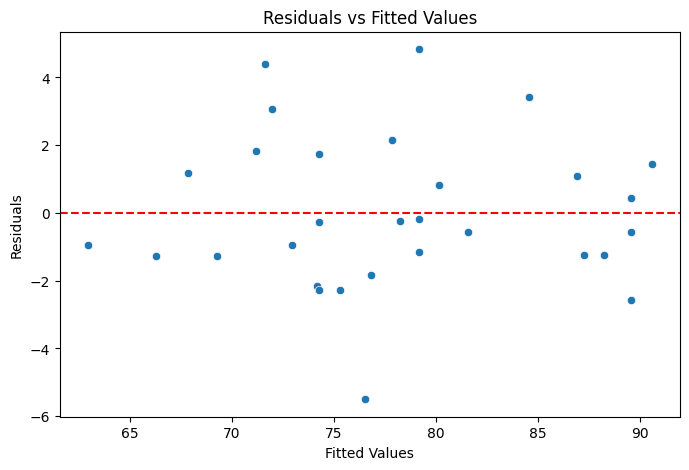
\includegraphics[width=0.5\textwidth]{assets/erros.png}
		      \caption{Interaction Graph}
	      \end{figure}
	      \begin{figure}[H]
		      \centering
		      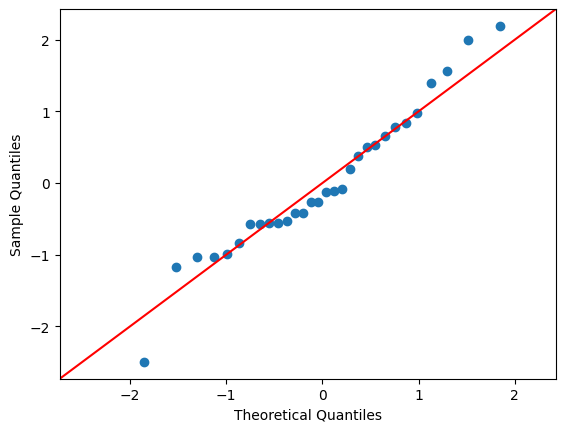
\includegraphics[width=0.5\textwidth]{assets/qqp.png}
		      \caption{Interaction Graph}
	      \end{figure}

	      Those show that the errors comes from a normal distribution with mean 0 and contrant variance. The qqp shows that the residuals are normally distributed

	\item  Plot the responses $Y_{ij}$ by blocks. What does this plot suggest about the appropriateness of the no-interaction assumption here?
	      \begin{figure}[H]
		      \centering
		      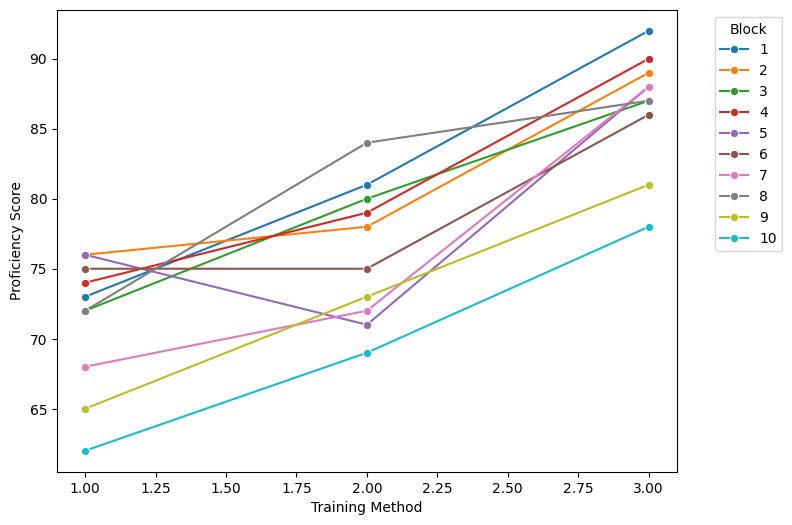
\includegraphics[width=0.5\textwidth]{assets/interaction.png}
		      \caption{Interaction Graph}
	      \end{figure}
	      The graph shows that there is interaction between the training methods
\end{enumerate}

Assume that the randomized block model is appropriate.
\begin{enumerate}[(a)]
	\item Test whether or not the mean proficiency is the same for the three training methods. Use a level of significance $\alpha = 0.05$. State the alternatives, decision rule, and conclusion. What is the p-value of the test?
	      \begin{table}[htbp]
		      \centering
		      \caption{ANOVA Table for Randomized Block Design}
		      \begin{tabular}{lrrrrr}
			      \toprule
			                & sum\_sq  & df   & mean\_sq & F       & PR(>F) \\
			      \midrule
			      C(Method) & 794.9333 & 2.0  & 397.4667 & 64.4565 & 0.0000 \\
			      C(Block)  & 579.9000 & 9.0  & 64.4333  & 10.4541 & 0.0000 \\
			      Residual  & 111.0000 & 18.0 & 6.1667   &         &        \\
			      \bottomrule
		      \end{tabular}
	      \end{table}
	      \begin{enumerate}
		      \item $H_0$: All treatments have the same effects
		      \item $H_1$: At least one treatment has an effect
	      \end{enumerate}

	      Given that the p-value is near 0 we reject the null hypothesis and conclude that there is significant differences between training methods
	\item Make all pairwise comparisons between the training method means; use the Tukey procedure with a 90\% confidence level coefficient. State your findings.
	      \begin{table}[htbp]
		      \centering
		      \caption{Tukey HSD Pairwise Comparisons Among Training Methods (90\% Confidence Level)}
		      \begin{tabular}{ccccccc}
			      \toprule
			      \textbf{Group 1} & \textbf{Group 2} & \textbf{Mean Diff} & \textbf{p-adj} & \textbf{Lower} & \textbf{Upper} & \textbf{Reject} \\
			      \midrule
			      1                & 2                & 4.9                & 0.0639         & 0.458          & 9.342          & \textbf{Yes}    \\
			      1                & 3                & 15.3               & 0.0000         & 10.858         & 19.742         & \textbf{Yes}    \\
			      2                & 3                & 10.4               & 0.0001         & 5.958          & 14.842         & \textbf{Yes}    \\
			      \bottomrule
		      \end{tabular}
	      \end{table}
	      \begin{enumerate}
		      \item $H_0$: There are no differences
		      \item $H_1$: The pair is different
	      \end{enumerate}
	      This table show that there are significant evidence to conclude that there is an effect on training method use and the score results. The order of the effect is
	      studding in Chicago then studding with the local office then studying at home. Overall this results make sense, this might be due to the level effort or investment the employee feels from the company.

	\item Test whether or not blocking effects are present; use \( \alpha = 0.05 \). State the alternatives, decision rule, and conclusion. What is the p-value of the test?
	      \begin{itemize}
		      \item \(H_0\) There is no blocking effects
		      \item \(H_1\) There is blocking effects
	      \end{itemize}


	      Since the p-value is less than 0.05, we reject the null hypothesis and conclude that there is a blocking effect

\end{enumerate}
\end{document}
